\documentclass[10pt]{beamer}
\usetheme{AGH}

\usepackage{lmodern}
\usepackage[utf8]{inputenc}
\usepackage{listings} 
\usepackage{siunitx}
\usepackage{filecontents,hyperref}
\usepackage{graphicx}
\usepackage{subcaption}
\usepackage{svg}

\usepackage{appendixnumberbeamer}
\usepackage{booktabs}
\usepackage{xspace}
\newcommand{\themename}{\textbf{\textsc{metropolis}}\xspace}

\renewcommand{\figurename}{Rys.}

\title{Drzewa wszystkich najkrótszych ścieżek - algorytm Dijkstry}
\subtitle{\normalsize{Aplikacja równoległa MPI}}
\date{}
\author{\normalsize{Arkadiusz Kasprzak, Aleksandra Poręba}}



\definecolor{lgray}{gray}{0.96}
\definecolor{lbcolor}{rgb}{0.9,0.9,0.9}
\lstset{
    framesep=2pt,
    basicstyle=\ttfamily,
    breaklines=true,
    breakatwhitespace=true,
    aboveskip={0.75\baselineskip},
    columns=fixed,
    showstringspaces=false,
    breaklines=true,
    prebreak = \raisebox{0ex}[0ex][0ex]{\ensuremath{\hookleftarrow}},
    frame=single,
    rulecolor=\color{lgray},
    showtabs=false,
    showspaces=false,
    showstringspaces=false,
    backgroundcolor=\color{lgray},
    identifierstyle=\ttfamily,
    keywordstyle=\color[rgb]{0,0,1},
    commentstyle=\color[rgb]{0.0,0.26,0.15},
    stringstyle=\color[rgb]{0.627,0.126,0.941}
}

\begin{document}

\titleframe[pl]

\begin{frame}
\frametitle{Agenda}
\tableofcontents
\end{frame}

\section{Algorytm Dijkstry - wprowadzenie}

\begin{frame}
\frametitle{Algorytm Dijkstry - wprowadzenie}
\begin{itemize}
\item Cel: znalezienie najkrótszych ścieżek z wybranego wierzchołka grafu do wszystkich pozostałych wierzchołków.
\item Operujemy na grafie skierowanym lub nieskierowanym o nieujemnych wagach krawędzi.
\item Algorytm zachłanny - w każdym kroku algorytmu wybierany jest wierzchołek o najmniejszej wartości kosztu.
\item Możliwość znalezienia zarówno najkrótszych ścieżek, jak i ich kosztów.
\end{itemize}
\end{frame}

\section{Budowa i działanie projektu}

\begin{frame}
\frametitle{Działanie projektu - wprowadzenie}
Program podzielony został na 3 części:
\begin{itemize}
\item 1 - inicjalizacja: wczytanie, walidacja i podział danych wejściowych, przygotowanie infrastruktury MPI, wykluczenie z dalszych części nadmiarowych procesów
\item 2 - wykonanie algorytmu przez wyznaczone do tego celu procesy
\item 3 - zapis wyników do pliku, zwolnienie zasobów MPI
\end{itemize}
Szczegółowy opis każdej z części wraz ze schematami blokowymi zawarty został w dokumentacji projektu.
\end{frame}

\begin{frame}
\frametitle{Działanie projektu - dane wejściowe}
\begin{itemize}
\item Dane podawane w postaci tzw. macierzy sąsiedztwa.
\item Dane wczytywane z pliku przez proces o numerze 0.
\end{itemize}
\begin{figure}
\centering
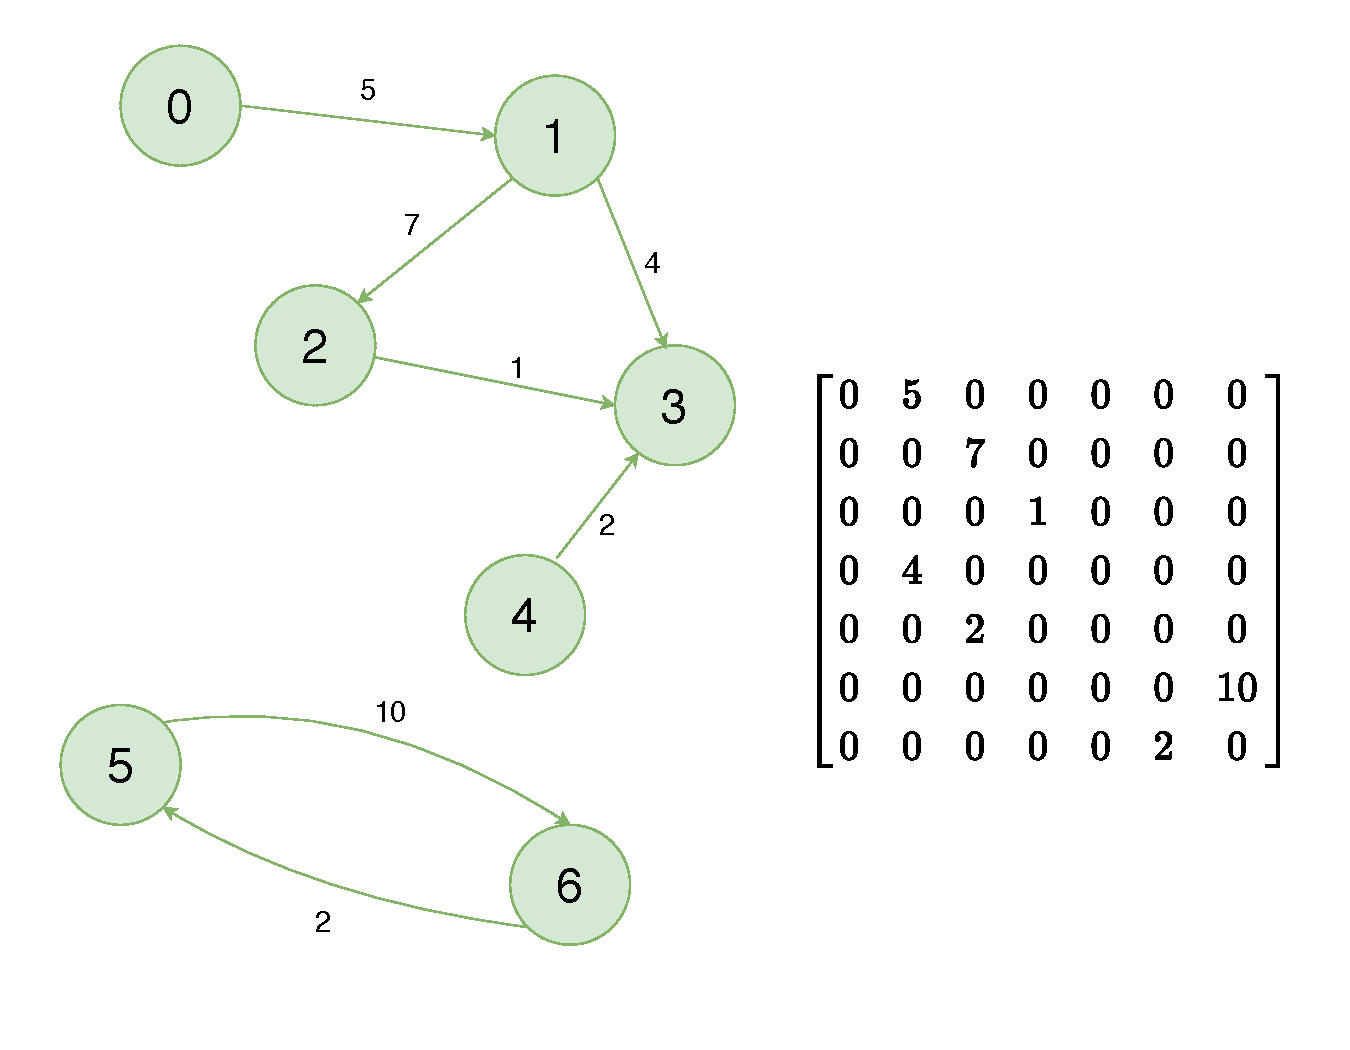
\includegraphics[width=0.7\textwidth]{static/Example.pdf}
\end{figure}

\end{frame}

\begin{frame}
\frametitle{Działanie projektu - podział danych wejściowych}
\begin{itemize}
\item Dane dzielone są kolumnami równomiernie pomiędzy wszystkie procesy. 
\item Jeśli podział równomierny niemożliwy, pozostałe $k$ kolumn dzielone jest między pierwsze $k$ procesów.
\item Procesy otrzymują następujące po sobie kolumny w formie tablic 1D.
\end{itemize}
\begin{figure}
\centering
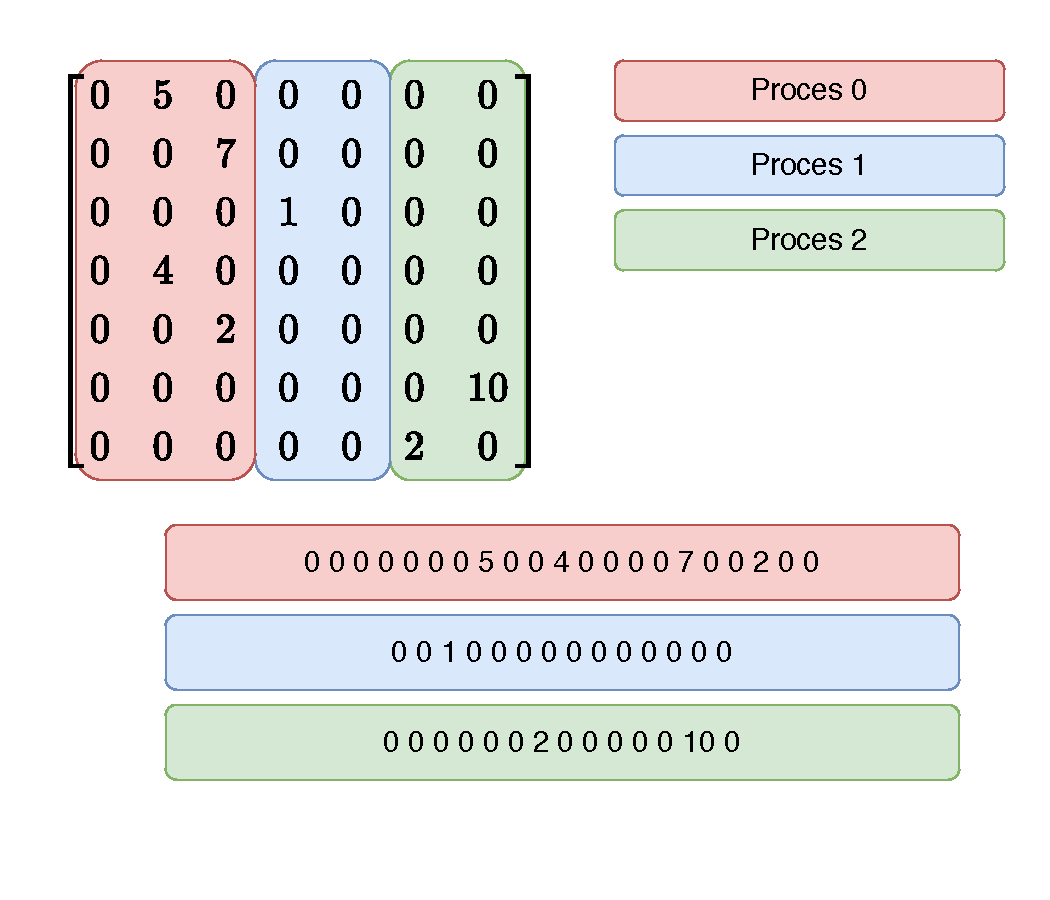
\includegraphics[width=0.5\textwidth]{static/MatrixChunks.pdf}
\end{figure}
\end{frame}


\begin{frame}
\frametitle{Działanie projektu - podział danych wejściowych}
\begin{itemize}
\item Jeśli liczba kolumn mniejsza niż liczba procesów, procesy nadmiarowe wykluczane z dalszego wykonywania algorytmu (poprzez podział komunikatora globalnego na dwie części)
\item Wykorzystane funkcjonalności MPI: \lstinline{MPI_Bcast}, \lstinline{MPI_Scatter}, \lstinline{MPI_Scatterv}, \lstinline{MPI_Comm_split}
\end{itemize}
\end{frame}

\begin{frame}
\frametitle{Działanie projektu - przebieg algorytmu}
\begin{itemize}
\item Operujemy na dwóch tablicach: $d$ - tablica kosztów, $p$ - tablica poprzedników
\item Każdy proces przechowuje swoją część tablicy, zgodnie z podziałem macierzy sąsiedztwa.
\item Tablica kosztów inicjalizowana nieskończonościami, tablica poprzedników - wartościami -1.
\item Koszt dla wierzchołka źródłowego ustawiany na 0.
\item Dodatkowo przechowujemy zbiór wierzchołków przetworzonych przez algorytm - początkowo jest on pusty.
\end{itemize}
\begin{figure}
\centering
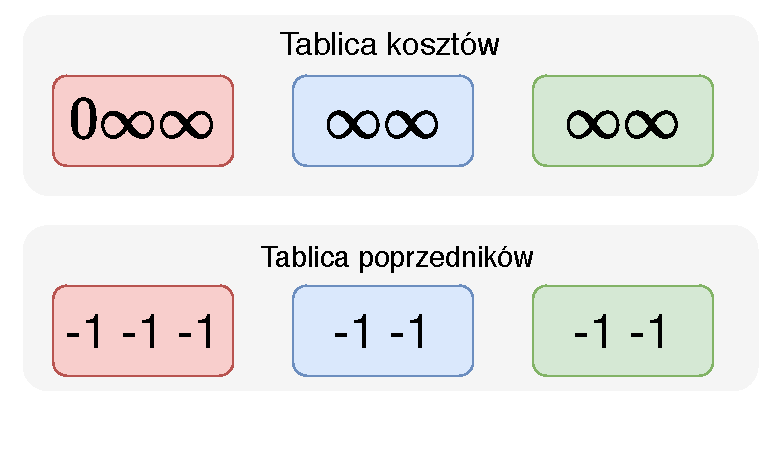
\includegraphics[width=0.35\textwidth]{static/Arrays.pdf}
\caption{Przykładowy początkowy stan tablic}
\end{figure}
\end{frame}

\begin{frame}
\frametitle{Działanie projektu - przebieg algorytmu}
W dalszej części powtarzamy poniższe czynności aż do momentu, gdy wspomniany zbiór zawierał będzie wszystkie wierzchołki:
\begin{itemize}
\item każdy proces spośród przydzielonych mu nieprzetworzonych jeszcze wierzchołków wybiera ten o najmniejszej wartości kosztu
\item spośród wybranych wierzchołków wyznaczany jest ten o globalnie najniższym koszcie (operacja \lstinline{MPI_Allreduce}). Zostaje on dodany do zbioru wierzchołków przetworzonych.
\item na podstawie wylosowanego wierzchołka przeprowadzana jest aktualizacja w tabelach kosztów i poprzedników
\end{itemize}
Po zakończeniu działania algorytmu fragmenty obu tablic są łączone za pomocą operacji \lstinline{MPI_Gatherv}. Wyniki algorytmu zapisywane są przez proces 0 do pliku.
\end{frame}

\begin{frame}
\frametitle{Działanie projektu - przebieg pojedynczej pętli}
Sytuacja początkowa. Niebieski - wierzchołek źródłowy. Czerwone linia - podział grafu. Na dole koszty.
\begin{figure}
\centering
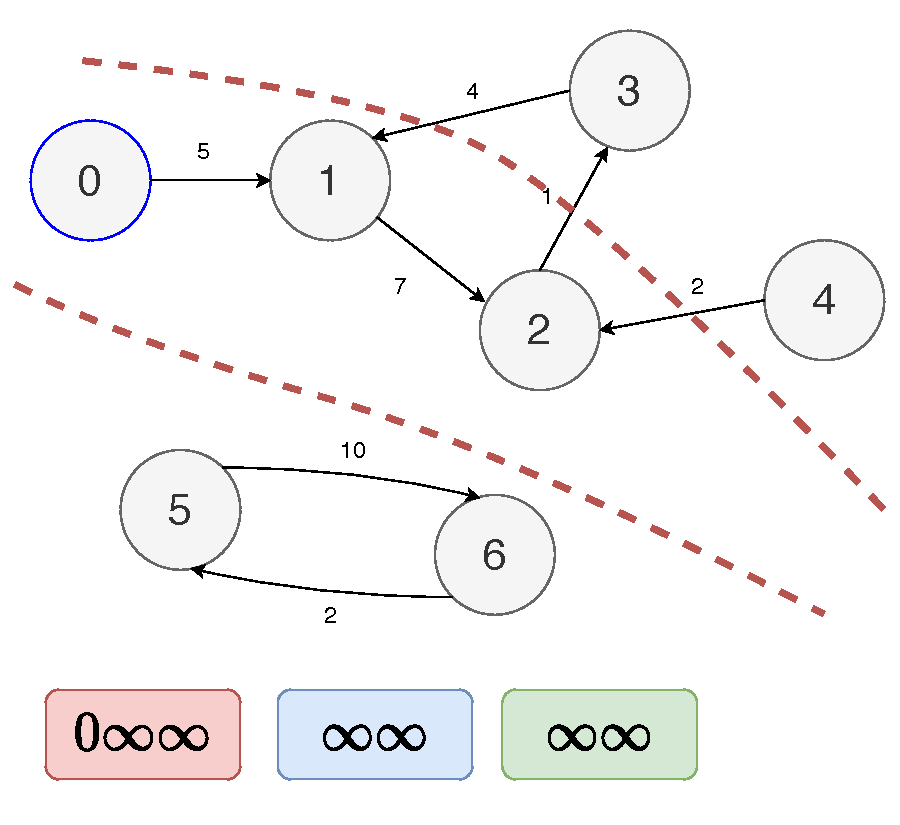
\includegraphics[width=0.6\textwidth]{static/Algo0.pdf}
\end{figure}
\end{frame}

\begin{frame}
\frametitle{Działanie projektu - przebieg pojedynczej pętli}
Wybór nieprzetworzonych wierzchołków o najniższym koszcie (w tablicy) w każdym z procesów.
\begin{figure}
\centering
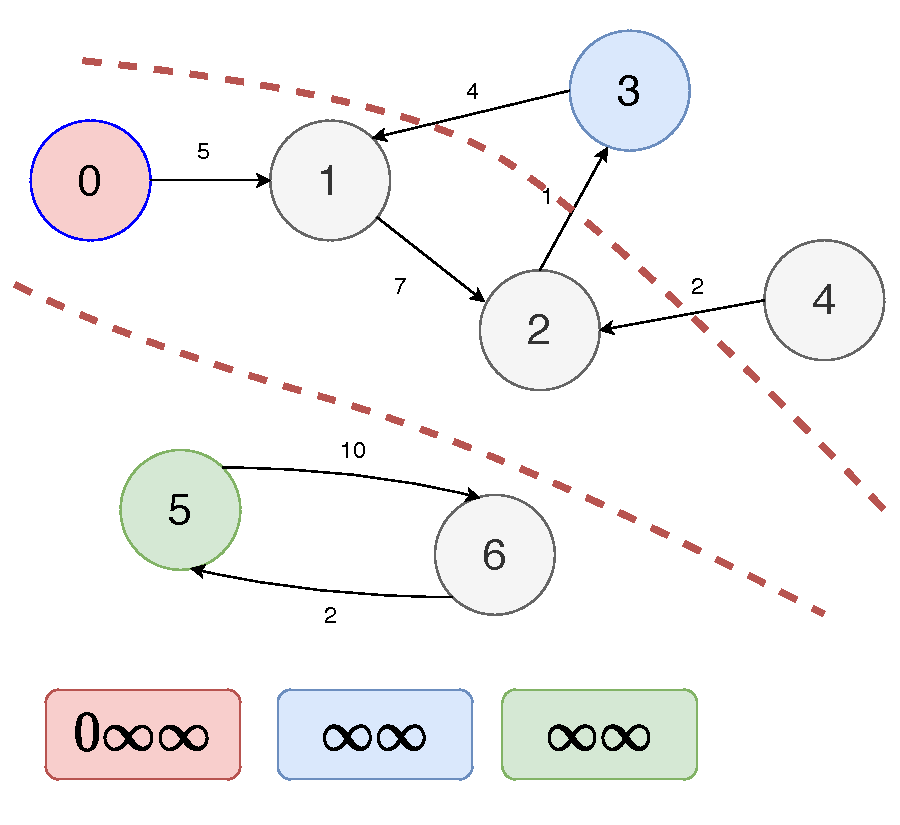
\includegraphics[width=0.6\textwidth]{static/Algo1.pdf}
\end{figure}
\end{frame}

\begin{frame}
\frametitle{Działanie projektu - przebieg pojedynczej pętli}
Wybór wierzchołka o globalnie najniższym koszcie (\lstinline{MPI_Allreduce}) i dodanie go do zbioru. Aktualizacja kosztów i poprzedników.
\begin{figure}
\centering
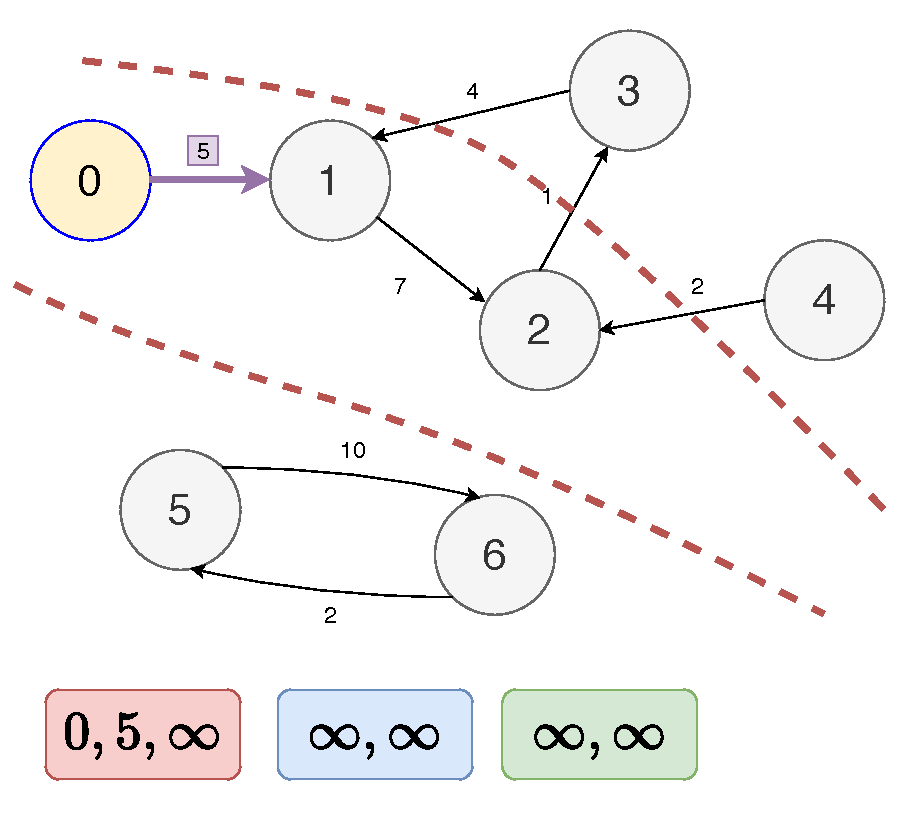
\includegraphics[width=0.6\textwidth]{static/Algo2.pdf}
\end{figure}
\end{frame}

\begin{frame}[fragile]
\frametitle{Interfejs}
\begin{itemize}
\item Podział grafu pomiędzy poszczególne procesy jest przedstawiany użytkownikowi.
\item Podobnie przedstawiany jest czas wykonywania się każdego z etapów programu (z punktu widzenia procesu 0).
\end{itemize}
\begin{lstlisting}[basicstyle=\tiny]
[Process 1] This process will handle 2 vertices in range [3, 4]
[Process 2] This process will handle 2 vertices in range [5, 6]
[Process 0] This process will handle 3 vertices in range [0, 2]
[Process 0] Total elapsed time: 0.0107225s
[Process 0] Setup took: 0.00937863s
[Process 0] Algorithm took: 0.000550448s
[Process 0] Printing solution took: 0.000793405s
\end{lstlisting}

\end{frame}


\begin{frame}
\frametitle{Komponenty projektu}
\begin{itemize}
\item \lstinline{DijkstraMPI} - implementacja równoległa algorytmu Dijkstry
\item \lstinline{DijkstraSerial} - implementacja sekwencyjna algorytmu Dijkstry
\item \lstinline{DijkstraCommon} - wspólna część obu implementacji, biblioteka statyczna
\end{itemize}
\begin{figure}
\centering
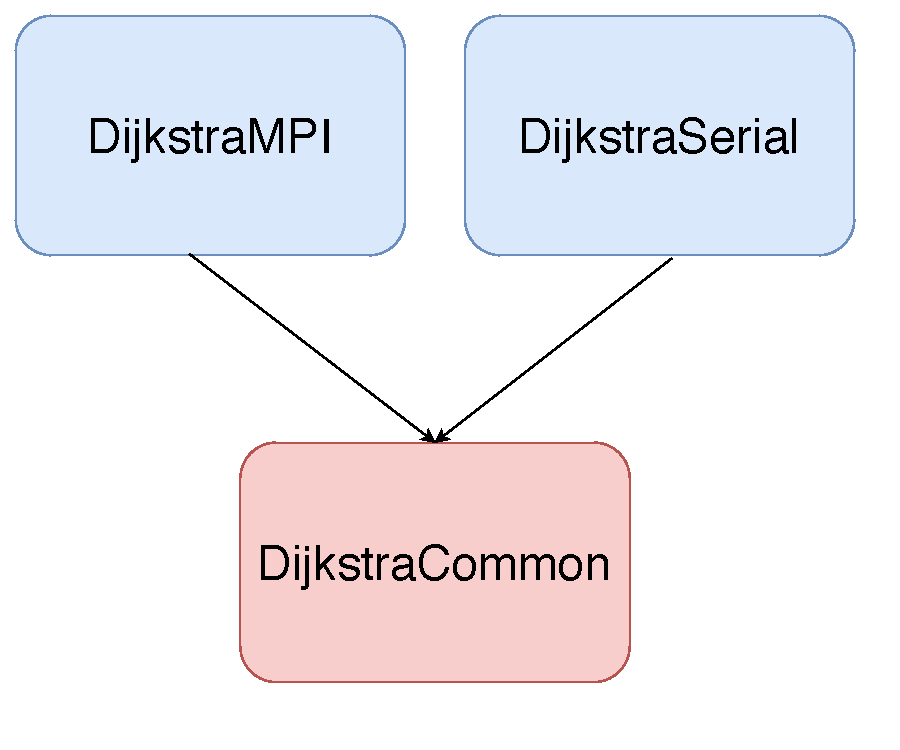
\includegraphics[width=0.4\textwidth]{static/DijkstraArch1.pdf}
\end{figure}

\end{frame}

\section{Przeprowadzone testy}

\begin{frame}
\frametitle{Testy wydajności}
Przeprowadzone zostały testy wydajności porównujące wersję sekwencyjną i równoległą projektu. W przypadku wersji równoległej przetestowano użycie 1, 4, 16 i 64 procesów.

\begin{figure}
\centering
\begin{subfigure}{.45\textwidth}
\centering
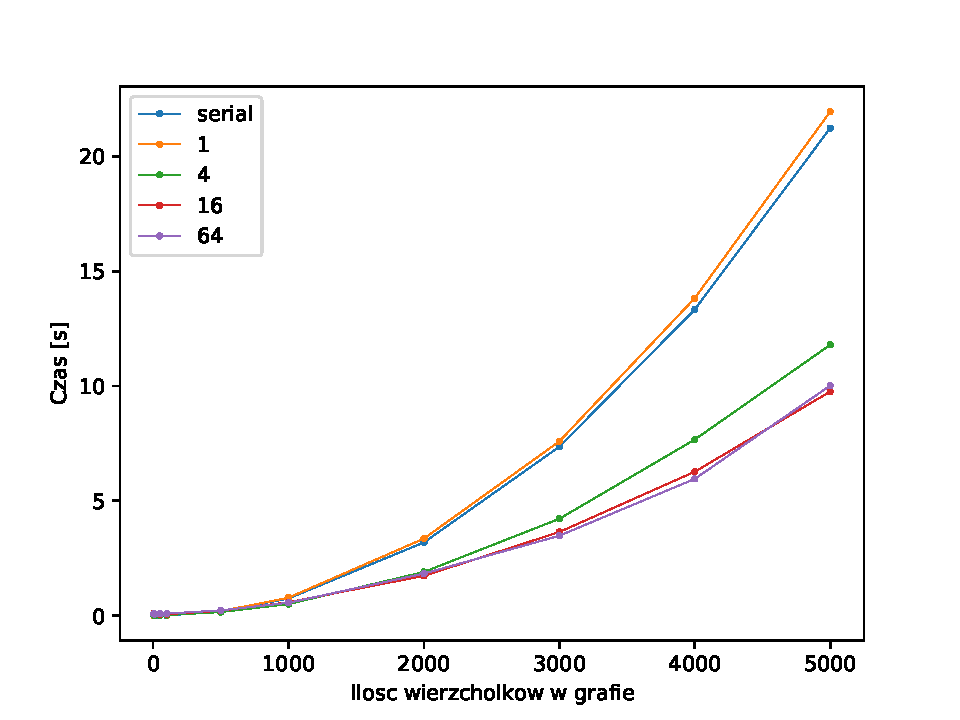
\includegraphics[width=\textwidth]{static/total_times.pdf}
\caption{Cały program}
\end{subfigure}
\begin{subfigure}{.45\textwidth}
\centering
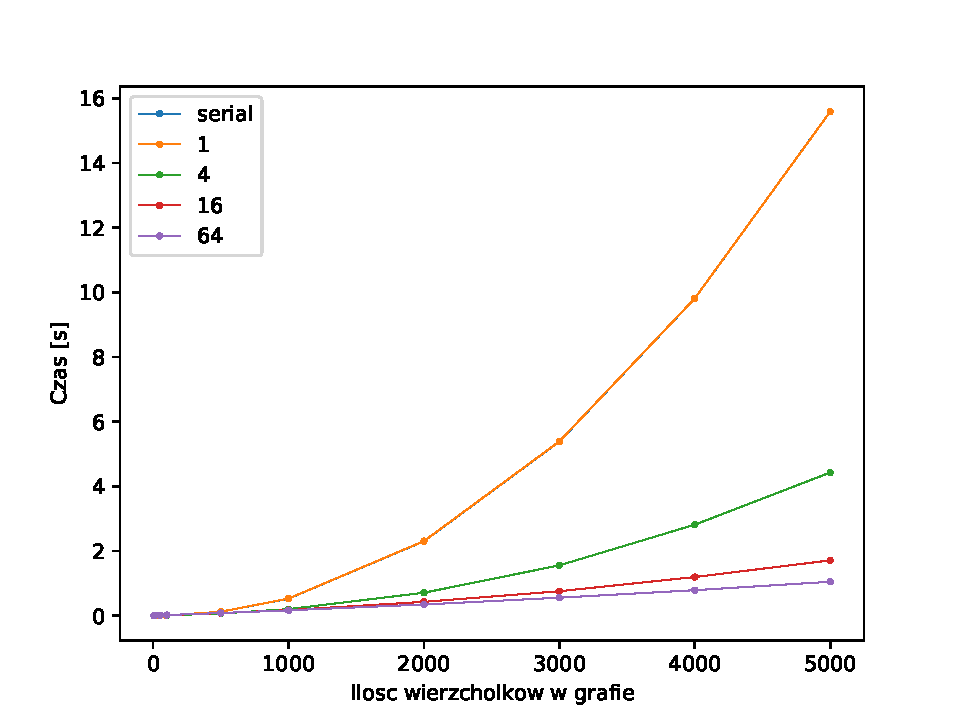
\includegraphics[width=\textwidth]{static/algo_times.pdf}
\caption{Część algorytmiczna}
\end{subfigure}
\end{figure}

\end{frame}

\section{Kompilacja i uruchomienie}

\begin{frame}
\frametitle{Kompilacja i uruchomienie}
\begin{itemize}
\item Przejście do katalogu \lstinline{build_uni}
\item Przygotowanie środowiska pracowni
\item Wykonanie polecenia \lstinline{make}
\item Wykonanie polecenia \lstinline{make runMPI} z opcjonalnymi argumentami określającymi: plik z węzłami, ilość procesów, numer wierzchołka źródłowego oraz ścieżkę do pliku z danymi
\item Wynik dostępny w pliku \lstinline{resultsMPI.txt}
\item Proces szczegółowo opisany w dokumentacji
\end{itemize}

\end{frame}

\end{document}